
\section{Exact Kernel Integration}
\label{appdx}

% \begin{figure}[ht]
% 	\begin{center}
% 		\epsfig{figure=./figures/fig_appendix.pdf,height=5cm}
% 	\end{center}
% 	\caption{Schematic of the mapped domain where numerical integration is performed.}
% 	\label{fig_appdx}
% \end{figure}

\begin{figure}[ht]

	\begin{center}
		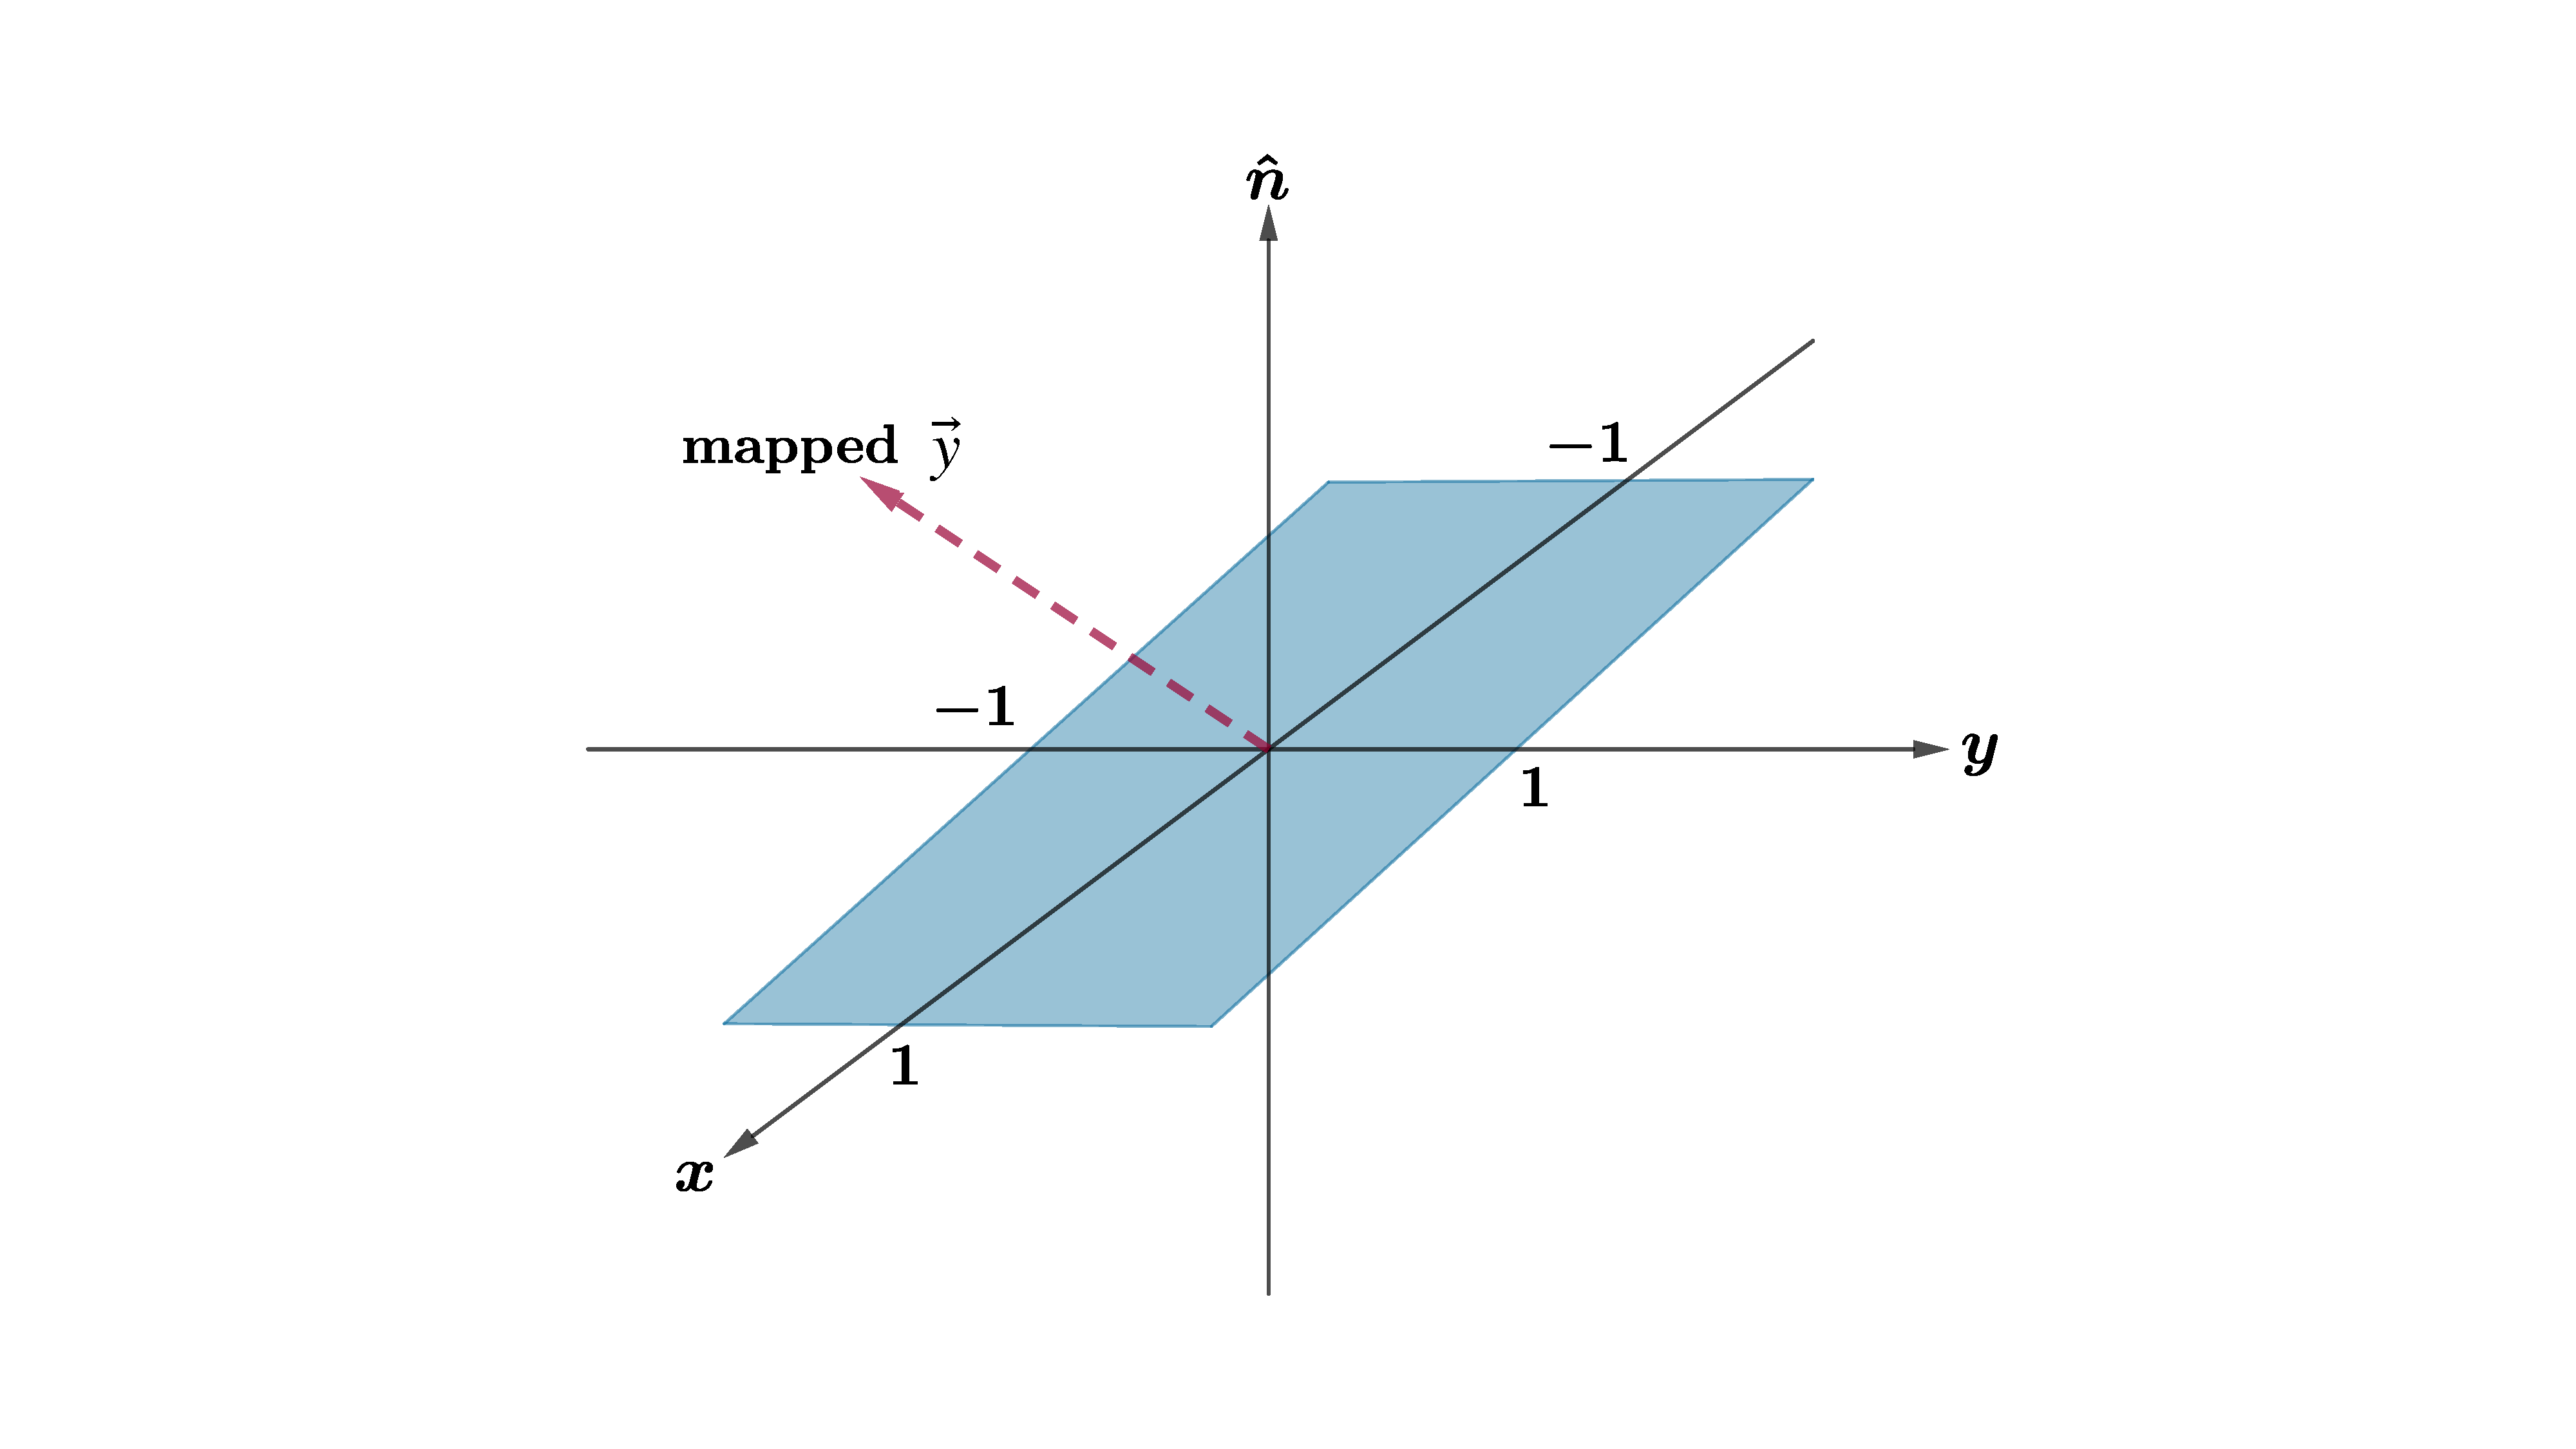
\includegraphics[scale=0.25]{figures/fig_appendix.pdf}

	\caption{Schematic of the mapped domain where numerical integration is performed.} 

\label{fig_appdx}
\end{center}
\end{figure}

When computing the flow around the aggregates, we need to integrate over square surfaces. 
To integrate over any square face, we first map the square over which we need to integrate to the square $(x,y,0)$ with $x \in [-1,1]$ and $y \in  [-1,1]$, as depicted in Fig. (\ref{fig_appdx}). The normal to the surface is thus always in the $z-$direction. We may then exactly evaluate all the surface integrals involved in either the single-layer or double-layer potential methods. 


\subsection{Single-layer potential}
\label{appdx_single}

In the single-layer potential approach, we need to compute integrals of the form
\begin{equation}
 \int_S  \left( \frac{\bar{\bar{I}}}{  ||\vec{x}-\vec{x}_0 ||  } + \frac{(\vec{x}-\vec{x}_0) (\vec{x}-\vec{x}_0) }{||\vec{x}-\vec{x}_0||^3} \right)  \ \text{d}S(\vec{x}) = \int_S   \frac{\bar{\bar{I}}}{  ||\vec{x}-\vec{x}_0 ||  }\text{d}S(\vec{x}) + \int_S   \frac{(\vec{x}-\vec{x}_0) (\vec{x}-\vec{x}_0) }{||\vec{x}-\vec{x}_0||^3}   \text{d}S(\vec{x}) = I_1 + I_2
 \label{eq_slp_int}.
\end{equation}
Here, we have that $ \vec{x} = (x,y,0)$ and we write $\vec{x}_0= (x_0,y_0,z_0)$ and
\[
 ||\vec{x}-\vec{x}_0||=R(x,y) = \sqrt{ (x-x_0)^2+(y-y_0)^2+z_0^2  }
\]
 We first consider the case when $x_0=y_0=z_0=0$, which arises when integrating over a face centered at the point where we are computing the velocity. In that case, we have $R(x,y) = \sqrt{x^2+y^2}$. We find for the diagonal terms of $I_1$
\begin{equation}
\int_{-1}^{1} \int_{-1}^{1} \frac{1}{   \sqrt{ x^2+y^2  }  }  \ \text{d}x \text{d}y = 8 \ \text{arcsinh}(1)
\end{equation}
and all the non-diagonal terms are zero. 

Away from the singularity, we can generally find antiderivatives, computed using Mathematica. For the integral $I_1$, we have
\begin{align}
\int_S \frac{1}{||\vec{x}-\vec{x}_0||}  \text{d}S(\vec{x})
& =
\int_{-1}^1 \int_{-1}^1  \frac{1   }{R(x,y)  } \ \text{d}x \text{d}y
\nonumber \\
&=
(x-x_0) \log \left(R(x,y) + (y-y_0)\right)
+(y-y_0)\log \left(R(x,y) +(x-x_0)   \right) \nonumber \\
&\left. \left. -z_0 \arctan \left(\frac{(x-x_0) (y-y_0)}{z_0 R(x,y) }\right)
+z_0 \arctan \left(\frac{(y-y_0)}{z_0}\right)
-(y-y_0)\right|_{x=-1}^1 \right|_{y=-1}^1 .
\label{eq_slp_const}
\end{align}

Note that there is no issue with evaluating the arctangent when $z_0=0$, as the multiplication by $z_0$ yields zero. Also, we need to be careful using this antiderivative when evaluating cases where $z_0=0$ and  $|x_0| = |y_0|=1$. In that case, the integral simplifies to 
\begin{equation}
\int_{-1}^{1} \int_{-1}^{1} \frac{1}{   \sqrt{ 1+x^2  }  }  \ \text{d}x \text{d}y = 4 \sinh^{-1}(1).
\end{equation}

Next, we consider the second part of integral equation (\ref{eq_slp_int}), $I_2$, which we index with $m$ and $n$
\begin{equation}
I_2 = \int_{-1}^1  \int_{-1}^1  \frac{(\vec{x}-\vec{x}_0)_m (\vec{x}-\vec{x}_0)_n }{R(x,y)^3}
	\ \text{d}x \text{d}y
.
\label{eq_slp_xx}
\end{equation}
Note that the numerator in equation (\ref{eq_slp_xx}), written in index notation,  refers to four different cases. There are two square-like terms
\begin{equation*}
\text{(a)} ~~~	(x-x_0)(x-x_0) ~~~ \text{or} ~~~	(y-y_0)(y-y_0)
	  ~~~\text{and (b)} ~~~ 	z_0^2,
\end{equation*}
and two mixed terms
\begin{equation*}
\text{(c)} ~~~	(x-x_0)(y-y_0)
	 ~~~ 	\text{and (d)} ~~~-(x-x_0)(z_0)
	 ~~~ \text{or} ~~~	-(y-y_0)(z_0).
\end{equation*}

Again, we treat $x_0=y_0=z_0=0$ separately. The first two diagonal terms (case (a)) are then
\begin{equation}
	\int _{-1}^1\int _{-1}^1
	\frac{x^2}{\left(x^2+y^2\right)^{3/2}}
	\ \text{d}x \text{d}y
	=4 \ \text{arcsinh}(1).
\end{equation}
The third diagonal term is zero because here $z_0=0$, and every non-diagonal term is zero by symmetry.

Assuming that $x_0y_0z_0\neq0$,  we consider cases (a)-(d) in turn.
For case (a), we have
\begin{align}
\int_{-1}^1 \int_{-1}^1 \frac{(x-x_0)^2 }{R(x,y)^{3}}  \ \text{d}x \text{d}y
&=(y-y_0) \left(\log \left(R(x,y)+x\right)-1\right) \nonumber \\ 
 &+z_0  \arctan\left(\frac{(y-y_0)}{z_0}\right) \left. \left.
-z_0 \arctan\left(\frac{(x-x_0)(y-y_0)}{ z_0R(x,y)}\right) \right|_{x=-1}^1 \right|_{y=-1}^1 .
\label{eq_slp_int_xx}
\end{align}
This case does not have evaluation issues since the argument of the logarithm can only be zero if $y=y_0$, which causes this entire term to be zero. Also, $R(x,y)$ can only be zero if $z_0=0$, which would then ensure that the third term would be zero. 
Note that the cases with numerator $(y-y_0)^2$ and  $(x-x_0)^2$ are equivalent if we swap the $x$ and $y$ variables by choosing a different mapping.


Case (b) is simpler since the $z_0$ term is constant. 
\begin{align}
\int_{-1}^1 \int_{-1}^1 \frac{z_0^2 }{R(x,y)^{3}}  \ \text{d}x \text{d}y
&= \left. \left.
z_0  \arctan \left(\frac{(x-x_0) (y-y_0)}{z_0  R(x,y)  }\right) \right|_{x=-1}^1 \right|_{y=-1}^1 
\label{eq_slp_int_zz}
\end{align}
Here, the only possibility to have an undefined value is when $z_0=0$, which simply gives a value of zero as the multiplying factor $z_0$ dominates the arctangent.


For case (c), we find
\begin{equation}
\int _{-1}^1\int _{-1}^1
\frac{(x-x_0)(y-y_0) }{R(x,y)^{3}}  \ \text{d}x \text{d}y
= \left. \left.
-R(x,y) \right|_{x=-1}^1 \right|_{y=-1}^1 .
\label{eq_slp_int_xy}
\end{equation}


Finally, for case (d), we have
\begin{equation}
\int_{-1}^1 \int_{-1}^1 \frac{(x-x_0) z_0 }{R(x,y)^{3}}  \ \text{d}x \text{d}y
= \left. \left.
-z_0 \log \left( R(x,y)+  (y-y_0)   \right) \ \right|_{x=-1}^1 \right|_{y=-1}^1 .
\label{eq_slp_int_xz}
\end{equation}
As before, this case also does not have any issue since $R(x,y)+(y-y_0)$ can only be zero if $z_0=0$, which causes the entire term to be zero.  

\subsection{Double-layer potential}

We now consider the double-layer potential integrals of the form
\begin{equation}
 \int_S
 \frac{(\vec{x}-\vec{x}_0)(\vec{x}-\vec{x}_0)     }{R(x,y)^5 }
\ (\vec{x}-\vec{x}_0) \cdot  n_k    \ \text{d}S(\vec{x}).
\label{eq_dlp_int}
\end{equation}
Since the inner product between the position and normal vectors always gives $z_0$ in the mapped coordinates, we focus on the integral,
\begin{equation}
\int_S
 \frac{(\vec{x}-\vec{x}_0)_m(\vec{x}-\vec{x}_0)_n     }{R(x,y)^5 }
    \ \text{d}S(\vec{x}).
\label{eq_dlp_int2}
\end{equation}
Note that we only need to compute this integral when $z_0\neq 0$, as otherwise equation (\ref{eq_dlp_int})  is zero because of the inner product. This also implies that $R(x,y)$ may never be zero.


We now consider the following four cases: \\ (a) $m=n=1$ or $m=n=2$, \\ (b) $m=n=3$, \\ (c) $m=1$, $n=2$ or $m=2$, $n=1$, \\ (d) $m=$1 or 2 and $n=3$, or $m=3$ and $n=$1 or 2 vice versa. 

For case (a), we find
\begin{align}
  \int_{-1}^1 \int_{-1}^1
  \frac{ (x-x_0)^2 }{R(x,y)^5 }
  \ \text{d}x \text{d}y
  =
  \frac{1}{3} 
  \biggl[
  &\frac{1}{z_0}\arctan \left(\frac{(x-x_0)(y-y_0)}{z_0 R(x,y)}\right) \biggr.
  \left. \left. \biggl. -\frac{(x-x_0) (y-y_0)}{\left((x-x_0)^2+z_0^2\right) R(x,y)}
  \biggr]   \ \right|_{x=-1}^1 \right|_{y=-1}^1 .
\label{eq_dlp_int_xx}
\end{align}
Since $z_0\neq0$ and $R(x,y) \neq 0$, there are no issues when evaluating this antiderivative. 

For case (b),
\begin{align}
\int_{-1}^1 \int_{-1}^1
\frac{ z_0^2     }{R(x,y)^5 }
\ \text{d}x \text{d}y
=
\frac{1}{3}
&\biggl[
\frac{1}{z_0}
\arctan \left(\frac{(x-x_0) (y-y_0)}{z_0 R(x,y)}\right)
\nonumber \\
& \left. \left. +\frac{(x-x_0) (y-y_0) \left(R(x,y)^2+ z_0^2\right)}{\left((x-x_0)^2+z_0^2\right) \left((y-y_0)^2+z_0^2\right) R(x,y)}
\biggr] \right|_{x=-1}^1 \right|_{y=-1}^1 ,
\label{eq_dlp_int_zz}
\end{align}
which again can always be evaluated directly when $z_0\neq0$.


Case (c) is relatively simple, as we can see, 
\begin{equation}
\int_{-1}^1 \int_{-1}^1
\frac{ (x-x_0)(y-y_0)    }{R(x,y)^5 }
\ \text{d}x \text{d}y
= \left. \left.
\frac{1}{3 R(x,y)} \right|_{x=-1}^1 \right|_{y=-1}^1 .
\label{eq_dlp_int_xy}
\end{equation}


Finally, case (d) is 
\begin{equation}
\int_{-1}^1 \int_{-1}^1
\frac{ (x-x_0)z_0    }{R(x,y)^5 }
\ \text{d}x \text{d}y
= \left. \left.
-\frac{(y-y_0) z_0}{3 \left((x-x_0)^2+z_0^2\right) R(x,y)} \right|_{x=-1}^1 \right|_{y=-1}^1.
\label{eq_dlp_int_xz}
\end{equation}
Once again, this is simple to evaluate when $z_0\neq0$.


\section{Extensional Flow past a Sphere}


In the case of a sphere of radius $R_s$, one may compute an exact solution for the flow satisfying $\vec{U}_{bg} = \bar{\bar{M}}\cdot \vec{x}$ at infinity and $\vec{U}_{bg} = 0$ on the surface of the sphere. 

The Stokes flow around the sphere is then \cite{guazzelli2012}
\[
\vec{u} = \left( \bar{\bar{M}} \cdot \vec{x} \right) \left( 1 - \frac{R_s^5}{r^5} \right) + \left( (\bar{\bar{M}} : \vec{x} \vec{x}) \vec{x} \right) \ \left( \frac{5}{2} \right)\left( \frac{R_s^5}{r^7}- \frac{R_s^3}{r^5} \right)
\]
and the corresponding pressure is
\[
P = - 5 \mu R_s^3  \frac{\bar{\bar{M}} : \vec{x}\vec{x}}{r^5}
\]
where $\vec{x}$ is the position vector and $r$ the distance to the center of the sphere. The stress tensor is then
\begin{eqnarray*}
\bar{\bar{T}} &=&  5 \mu R_s^3  \frac{\bar{\bar{M}} : \vec{x}\vec{x}}{r^5} + 2 \bar{\bar{M}} \left( 1 - \frac{R_s^5}{r^5} \right).+ ( \vec{x} (\bar{\bar{M}} \cdot \vec{x})  +  (\bar{\bar{M}} \cdot \vec{x}) \vec{x} ) \left( \frac{10R_s^5}{r^7} - \frac{5R_s^3}{r^5} \right)  \\
& & + 5 \left( \frac{R_s^5}{r^7}- \frac{R_s^3}{r^5} \right) (\bar{\bar{M}} : \vec{x}\vec{x}) \bar{\bar{I}} +  5 \left( \frac{5R_s^3}{r^7}- \frac{7R_s^5}{r^9} \right) (\bar{\bar{M}} : \vec{x}\vec{x}) \vec{x} \vec{x}
\end{eqnarray*}

On the surface of the sphere, where $r=R_s$, we consider the stress vector, $\vec{f} = \bar{\bar{T}}\cdot \hat{n}$, where $\hat{n} = \vec{x}/R_s$, and find
\[
\vec{f} = \left.  \bar{\bar{T}} \cdot \hat{n} \right|_{r=R_s}  = \frac{5 \mu}{R_s^2} \left( \frac{2 \bar{\bar{M}}: \vec{x} \vec{x}}{R_s} -  \frac{2 \bar{\bar{M}}: \vec{x} \vec{x}}{R_s} + \bar{\bar{M}} \cdot \vec{x} R_s  \right) = \frac{5 \mu \bar{\bar{M}} \cdot \vec{x}}{R_s}
\]

For an eigenvector $\hat{v}_i$ with eigenvalue $\lambda_i$, we thus find
\[
S_i  = \frac{1}{2} \int_S | \vec{f} \cdot \vec{v}_i | \ dS = 5  \pi \mu R_s^2 \lambda_i .
\]

